\documentclass[10pt,aspectratio=169,serif]{beamer}

\usepackage[fontset=none, scheme=plain]{ctex}
\IfFontExistsTF{Songti SC}{%
	\setCJKmainfont{Songti SC}[AutoFakeSlant=0.2]%
	\setCJKsansfont{Songti SC}[AutoFakeSlant=0.2]%
}{%
	\setCJKmainfont{FandolSong-Regular}[Extension=.otf,BoldFont=FandolSong-Bold,AutoFakeSlant=0.2]%
	\setCJKsansfont{FandolSong-Regular}[Extension=.otf,BoldFont=FandolSong-Bold]%
}
\usepackage{amsmath,amssymb,graphicx,tikz,booktabs,multicol,calligra}
\usepackage{pgfplots}
\pgfplotsset{compat=1.18}
\usepackage{tcolorbox}
\tcbuselibrary{skins}
\usepackage{XyygU}
\usepackage{caption}
\captionsetup[figure]{name=图,labelsep=period}

\usetikzlibrary{arrows.meta,positioning,calc}

% 公式间距
\setlength{\abovedisplayskip}{0pt plus 2pt minus 2pt}
\setlength{\belowdisplayskip}{0pt plus 2pt minus 2pt}

\title[习题1.2]{习题 1.2}
\subtitle{集合间的基本关系}
\author{}
\institute{}
\date{2026-10-16}

\begin{document}

\begin{frame}
  \titlepage
\end{frame}

% ========== 第1题 ==========
\begin{frame}[t]{第1题：选用适当符号填空}
\textbf{1.} 选用适当的符号填空：

\vspace{0.4em}
(1) 若集合 $A = \{x \mid 2x - 3 < 3x\}$，$B = \{x \mid x \ge 2\}$，则
\[
-4\ \underline{\hspace{0.8em}}\ B,\ \ -3\ \underline{\hspace{0.8em}}\ A,\ \ \{2\}\ \underline{\hspace{0.8em}}\ B,\ \ B\ \underline{\hspace{0.8em}}\ A;
\]

(2) 若集合 $A = \{x \mid x^2 - 1 = 0\}$，则
\[
1\ \underline{\hspace{0.8em}}\ A,\ \ \{-1\}\ \underline{\hspace{0.8em}}\ A,\ \ \varnothing\ \underline{\hspace{0.8em}}\ A,\ \ \{1,-1\}\ \underline{\hspace{0.8em}}\ A;
\]

(3) $\{x \mid x \text{ 是菱形}\}$ \underline{\hspace{0.8em}} $\{x \mid x \text{ 是平行四边形}\}$；

\qquad $\{x \mid x \text{ 是等腰三角形}\}$ \underline{\hspace{0.8em}} $\{x \mid x \text{ 是等边三角形}\}$。
\end{frame}

\begin{frame}[t]{第1题 解答}
\begin{tcolorbox}[colback=orange!10,colframe=orange,title=\textbf{解}]
先化简：$A = \{x \mid 2x-3 < 3x\} = \{x \mid x > -3\}$，$B = \{x \mid x \ge 2\}$。

\vspace{0.3em}
\textbf{(1)} $-4 \notin B$（$-4 < 2$）；$-3 \notin A$（$-3$ 不大于 $-3$）；$\{2\} \subsetneqq B$；$B \subsetneqq A$（$B$ 的元素都满足 $x>-3$，但 $0 \in A$ 而 $0 \notin B$）。

\vspace{0.3em}
\textbf{(2)} $A = \{-1, 1\}$。故 $1 \in A$；$\{-1\} \subsetneqq A$；$\varnothing \subsetneqq A$；$\{1,-1\} = A$。

\vspace{0.3em}
\textbf{(3)} 菱形是特殊的平行四边形，故 $\{$菱形$\} \subsetneqq \{$平行四边形$\}$；

等边三角形是特殊的等腰三角形，故 $\{$等腰三角形$\} \supsetneqq \{$等边三角形$\}$。
\end{tcolorbox}
\end{frame}

% ========== 第2题 ==========
\begin{frame}[t]{第2题：集合关系与Venn图}
\textbf{2.} 指出下列各集合之间的关系，并用 Venn 图表示：

\vspace{0.5em}
\[
A = \{x \mid x \text{ 是四边形}\},\quad
B = \{x \mid x \text{ 是平行四边形}\},
\]
\[
C = \{x \mid x \text{ 是矩形}\},\quad
D = \{x \mid x \text{ 是正方形}\}.
\]
\end{frame}

\begin{frame}[t]{第2题 解答与Venn图}
\begin{tcolorbox}[colback=orange!10,colframe=orange,title=\textbf{解}]
从属关系：正方形 $\subsetneqq$ 矩形 $\subsetneqq$ 平行四边形 $\subsetneqq$ 四边形。

即：$\alert{D \subsetneqq C \subsetneqq B \subsetneqq A}$。

\vspace{0.5em}
\begin{center}
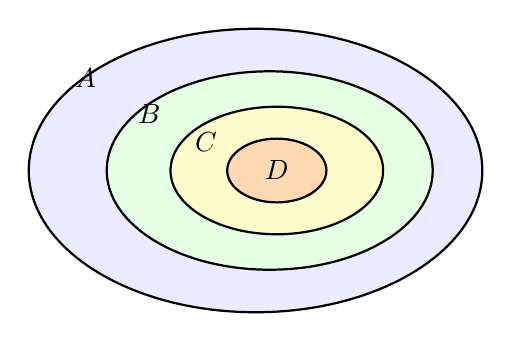
\begin{tikzpicture}[scale=0.9]
  \draw[thick,fill=blue!8] (0,0) ellipse (3.2 and 2.0);
  \draw[thick,fill=green!10] (0.2,0) ellipse (2.3 and 1.4);
  \draw[thick,fill=yellow!20] (0.3,0) ellipse (1.5 and 0.9);
  \draw[thick,fill=orange!30] (0.3,0) ellipse (0.7 and 0.45);
  \node at (-2.4,1.3) {$A$};
  \node at (-1.5,0.8) {$B$};
  \node at (-0.7,0.4) {$C$};
  \node at (0.3,0) {$D$};
\end{tikzpicture}
\end{center}
{\small 外到内依次为：四边形 $A$、平行四边形 $B$、矩形 $C$、正方形 $D$。}
\end{tcolorbox}
\end{frame}

% ========== 第3题 ==========
\begin{frame}[t]{第3题：举子集}
\textbf{3.} 举出下列各集合的一个子集：

\vspace{0.8em}
\begin{columns}
\begin{column}{0.55\textwidth}
(1) $A = \{x \mid x \text{ 是立德中学的学生}\}$；

(3) $C = \{0\}$；
\end{column}
\begin{column}{0.45\textwidth}
(2) $B = \{x \mid x \text{ 是三角形}\}$；

(4) $D = \{x \in \mathbf{Z} \mid 3 < x < 30\}$。
\end{column}
\end{columns}
\end{frame}

\begin{frame}[t]{第3题 解答}
\begin{tcolorbox}[colback=orange!10,colframe=orange,title=\textbf{参考答案（不唯一）}]
\textbf{(1)} 任取立德中学的一名学生即可，例如 $\{$立德中学高一（1）班的学生$\}$。

\vspace{0.5em}
\textbf{(2)} 任取一类三角形即可，例如 $\{$等边三角形$\}$ 或 $\{$直角三角形$\}$。

\vspace{0.5em}
\textbf{(3)} $C = \{0\}$ 的子集为：$\varnothing$ 和 $\{0\}$。

\vspace{0.5em}
\textbf{(4)} $D = \{4, 5, 6, \dots, 29\}$，任取其中一部分即可，例如 $\{4, 5, 6\}$ 或 $\{x \in \mathbf{Z} \mid 3 < x < 10\}$。
\end{tcolorbox}
\end{frame}

% ========== 第4题 ==========
\begin{frame}[t]{第4题：点集之间的关系}
\textbf{4.} 在平面直角坐标系中，集合 $C = \{(x,y) \mid y = x\}$ 表示直线 $y = x$。从这个角度看，集合
\[
D = \left\{(x,y) \,\middle|\, \begin{cases} 2x - y = 1,\\ x + 4y = 5 \end{cases}\right\}
\]
表示什么？集合 $C$，$D$ 之间有什么关系？
\end{frame}

\begin{frame}[t]{第4题 解答}
\begin{tcolorbox}[colback=orange!10,colframe=orange,title=\textbf{解}]
解方程组：
\[
\begin{cases}
2x - y = 1,\\
x + 4y = 5.
\end{cases}
\quad\Rightarrow\quad
\begin{cases}
y = 2x - 1,\\
x + 4(2x - 1) = 5,
\end{cases}
\]
\[
9x = 9 \quad\Rightarrow\quad x = 1,\ \ y = 1.
\]

所以 $D = \{(1,\ 1)\}$，它表示坐标为 $(1,1)$ 的一个点。

\vspace{0.5em}
又因为点 $(1,1)$ 的坐标满足 $y = x$，即 $(1,1) \in C$，所以 $D$ 是 $C$ 的真子集：
\[
\alert{D \subsetneqq C}.
\]
\end{tcolorbox}
\end{frame}

% ========== 第5题 ==========
\begin{frame}[t]{第5题：集合相等与子集求参数范围}
\textbf{5.}

(1) 设 $a,\ b \in \mathbf{R}$，$P = \{1,\ a\}$，$Q = \{-1,\ -b\}$，若 $P = Q$，求 $a - b$ 的值；

\vspace{0.8em}
(2) 已知集合 $A = \{x \mid 0 < x < a\}$，$B = \{x \mid 1 < x < 2\}$，若 $B \subseteq A$，求实数 $a$ 的取值范围。
\end{frame}

\begin{frame}[t]{第5题 解答}
\begin{tcolorbox}[colback=orange!10,colframe=orange,title=\textbf{解}]
\textbf{(1)} 由 $P = Q$，两集合元素必须完全相同。

$P$ 含元素 $1$ 和 $a$，$Q$ 含元素 $-1$ 和 $-b$。

注意 $1 \ne -1$，故只能 $1 = -b$ 且 $a = -1$，即 $b = -1$，$a = -1$。

所以 $a - b = -1 - (-1) = \alert{0}$。

\vspace{0.8em}
\textbf{(2)} $B = \{x \mid 1 < x < 2\}$ 是 $A = \{x \mid 0 < x < a\}$ 的子集，意味着区间 $(1,2)$ 必须完全落在区间 $(0,a)$ 内。

画数轴可知：左端 $0 < 1$ 已满足；右端要求 $a \ge 2$（若 $a = 2$，则 $(0,2)$ 仍包含 $(1,2)$）。

\vspace{0.3em}
故实数 $a$ 的取值范围为 $\alert{a \ge 2}$，即 $[2,\ +\infty)$。
\end{tcolorbox}
\end{frame}

\begin{frame}[c]
  \begin{center}
    {\Huge\calligra Thanks!}
  \end{center}
\end{frame}

\end{document}
